% Document title
% ==============
% Draft for conference/workshop paper to be submitted to http://tappcs.blogspot.mx/
% 2--4 pages in Spanish or English.

\documentclass[10pt,conference,a4paper]{IEEEtran}
\usepackage[utf8x]{inputenc}
\usepackage[hidelinks]{hyperref}
\usepackage{graphicx}
\usepackage{pgfplots}
\usepackage[T1]{fontenc}
\bibliographystyle{IEEEtran}

% This enables the kanji in the table, but all typefaces turn uglier.
% Also must be generated with xelatex
%\usepackage{xeCJK}
%\setCJKmainfont{cyberbit.ttf}


\title{Some Nice Title Goes Here, Eventually\ldots}

\author{
	\IEEEauthorblockN{Lars Fredrik Karlstr\"om}
	\IEEEauthorblockA{Faculty of Science, Dept. of Computer Science\\ Universidad Aut\'onoma de Baja California\\ \href{mailto:fredrik.karlstrm@uabc.edu.mx}{\texttt{fredrik.karlstrm@uabc.edu.mx}}}
	\and
	\IEEEauthorblockN{Everardo Guti\'errez L\'opez}
	\IEEEauthorblockA{Faculty of Science, Dept. of Computer Science\\ Universidad Aut\'onoma de Baja California\\ \href{mailto:everardo.gutierrez@uabc.edu.mx}{\texttt{everardo.gutierrez@uabc.edu.mx}}}
}

\pgfplotsset{
	compat = newest,
	xlabel near ticks,
	ylabel near ticks
}

\begin{document}
	\maketitle

	\begin{abstract}
		Handwriting continues to play a significant role in daily life, warranting continued research in the field of intelligent character recognition.
		Due to their vast number of symbols, east asian scripts such as Japanese remain challenging to process efficiently with high accuracy.
		In this work, we formulate a modular design scheme based on reviews of previous work and the characteristics of the Japanese kanji sinographs.
		We also describe an ongoing effort to implement and evaluate a basic proof-of-concept handwriting recognition system based on artificial neural networks.


	\end{abstract}
	\medskip
	\begin{IEEEkeywords}
		Intelligent character recognition, handwriting recognition, kanji recognition, artificial neural network.
	\end{IEEEkeywords}

	\section{Introduction}
	\label{sec:introduction}

	Although a variety of efficient digital input methods have become all but second nature to recent generations, for the vast majority
	handwriting remains an integral activity in daily life.
	The importance to further improve upon the state-of-the-art in handwriting recognition is underlined not only by the continued prevalence of 
	handwriting, but also by the need to digitalize archived material, the significant role of handwriting in the development of fine motor skills,
	and a variety of other areas of application, such as signature verification. \cite{plamondon2000online}

	As an area of research, handwriting recognition predates even the digital computer. In 1888, Elisha Gray was awarded a patent %\cite{gray1888telautograph}
	for the ``Telautograph,'' which is considered a precursor to the stylus and digitizer, and in
	a 1957 publication, T. L. Dimond summarized early character recognition efforts and introduced the Stylator, an early input recognition device. \cite{dimond1957devices}
	
	The decades of research since has introduced a vast number of recognition techniques for writing in any and all forms. Noteworthy successful techniques in
	widespread use today include support vector machines, hidden Markov models, and artificial neural networks. \cite{fujisawa2008forty, tappert1990state}

	This paper documents a work in progress on the topic of intelligent handwriting recognition of Japanese characters.
	The remainder of the article is structured as follows:
	In section \ref{sec:problem_description} we present the Japanese writing system and outline the primary issues with handwriting recognition for east asian script;
	in section \ref{sec:previous_work}, we discuss some notable advances aimed at solving various aspects of the aforementioned problems.

	An explanation of our solution approach is given in section \ref{sec:proposed_solution}, and an experimental implementation is described in section \ref{sec:experiments}
	along with some initial observations. Finally, planned future work is presented in section \ref{sec:future_work}, whereafter we conclude by summarizing the
	contents of this paper in section \ref{sec:summary}.

	
	\begin{figure}
		\centering
		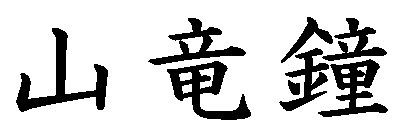
\includegraphics[width=2.75in]{./fig/yama-ryuu-kane.eps}
		\caption{Sample characters. The kanji ``yama'' (mountain), ``ry\=u'' (dragon), and ``kane'' (bell), written with 3, 10, and 20 strokes, respectively.}
		\label{fig_kanji_sample}
	\end{figure}



	\section{Problem description}
	\label{sec:problem_description}

	Any form of digital handwriting recognition is a complex undertaking,
	where the performance of the system is impacted by a multitude of factors---spanning
	everything from the quality and quantity of training data, to resilience toward input
	translation, rotation, and noise. As the number of candidate categories increase
	the size of the search space, however, the task quickly grows monumental.

	The Japanese writing system consists of the two \emph{kana} syllabaries \emph{hiragana} and \emph{katakana},
	as well as the sinographs commonly known as \emph{kanji}---literally ``Han characters''---that stem from China.
	The Japanese Ministry of Education's official ``regular use'' (j\=oy\=o) kanji list defines a set of 2,136
	baseline characters taught in elementary and secondary education. \cite{hadamitzky2012japanese}
	This set is far from exhaustive, though: the Japanese Industrial Standard X 0208 encoding, for instance, contains 6,355 different kanji.

	Although the characters are vast in number and differ significantly from one another in terms of complexity (see figures \ref{fig_kanji_sample}
	and \ref{fig_kanji_stroke_hist}), the writing system itself is not arbitrary. Any kanji may be broken down into smaller units, known as graphemes, 
	and they are commonly ``classified'' by basic, frequently ocurring components referred to as radicals.
	Furthermore, stroke order is dictated by a set of rules. In essence, kanji are written from top to bottom and left to right within imagined squares. \cite{foerster1994kanji}

	These properties are often leveraged in kanji recognition systems, but not without penalty: relying on the correct stroke order during online
	recognition, for instance, severely impacts recognition rates when a user provides erroneous input---even though it may still be \emph{visually} correct. \cite{shin2002optimal}

	While certain aspects such as noise reduction and normalization remain similar across systems, the characteristics mentioned above result in
	recognition systems designed for western input not performing satisfactorily when applied to east asian script \cite{jager2003state, tappert1990state}%, liu2004online}
	---unless the solution relies on complex techniques such as  ``deep'' neural networks. \cite{ciresan2012multi}


	%Given that the category search space for Japanese characters is an order of magnitude larger and contains a vastly differing set of
	%characteristics than its western counterparts, the same designs that yield highly accurate results on 
	%western handwriting recognition tasks do not perform satisfactorily when applied to asian script \cite{jager2003state, tappert1990state, liu2004online}
	%-- unless the solution relies on complex and computationally expensive techniques, such as  ``deep'' neural networks. \cite{ciresan2012multi}


	\begin{figure}
		\centering
		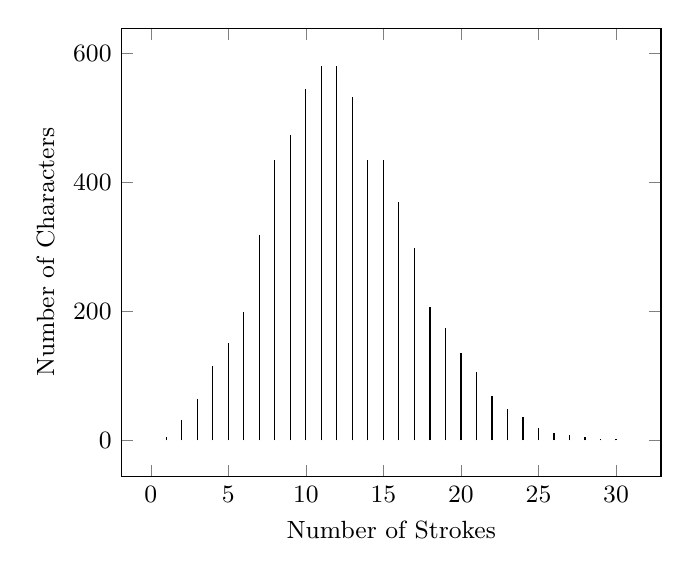
\begin{tikzpicture}[font=\small]
			\begin{axis}[
				ycomb,
				xlabel={Number of Strokes},
				ylabel={Number of Characters},
			]
				%\addplot[fill=white] coordinates {
				\addplot [] coordinates {
					(1, 6)
					(2, 32)
					(3, 64)
					(4, 115)
					(5, 151)
					(6, 199)
					(7, 318)
					(8, 434)
					(9, 473)
					(10, 544)
					(11, 581)
					(12, 581)
					(13, 532)
					(14, 435)
					(15, 434)
					(16, 369)
					(17, 299)
					(18, 207)
					(19, 175)
					(20, 135)
					(21, 106)
					(22, 69)
					(23, 49)
					(24, 37)
					(25, 20)
					(26, 12)
					(27, 8)
					(28, 6)
					(29, 3)
					(30, 2)
				};
			\end{axis}
		\end{tikzpicture}
		\caption{Distribution of 6,400 kanji by stroke count. Min = 2, Max = 581. \emph{Data source: KanjiVG.} \cite{kanjivg}}
		\label{fig_kanji_stroke_hist}
	\end{figure}



	\section{Previous work}
	\label{sec:previous_work}

	A vast body of work has been amassed on the topic of Japanese handwriting recognition.
	Here we present a summary of publications dealing with our principal issues of interest,
	and whose findings motivates our proposal.
	%Here we summarize some notable publications that influenced our adopted approach.


	In \cite{joe1989large}, Mori and Joe present ``selective'' and ``integrative'' neural networks that 
	segment categories into small groups, thereby improving the recognition rate of each network.

	
	After structuring the search space by clustering, Yang et al. perform two-stepped offline recognition by first
	comparing the input character to the centroids of each cluster, and then distinguishing between the members of the cluster
	whose centroid most closely matched the input. \cite{yang2003accelerating}


	In \emph{Hybrid Pen-Input Character Recognition System Based on Integration of Online-Offline Recognition},
	the authors present a system that leverages the advantages provided by each type of recognition.
	In addition to a discussion of various integration techniques, two feature extraction methods are described in detail: 
	a gradient-based technique for offline input, and a recursive substroke extractor for online input.


	% Got A-H classification from here
	In \cite{nakai2001substroke}, the authors adapt a continuous speech recognition algorithm utilizing
	hidden Markov models for the purpose of online kanji recognition. Captured strokes are segmented into
	substrokes and classified based on directionality (see figure \ref{fig_stroke_categories});
	the resulting vector elements are thereafter employed as dictionary search keys.


	\emph{Online Handwritten Kanji Recognition Based on Inter-Stroke Grammar} explains the hierarchical structure of kanji,
	and explores how to leverage this information using stochastic context-free grammars. \cite{ota2007online}

	Finally, albeit not directly applied to Japanese handwriting recognition, \emph{Best Practices for Convolutional Neural Networks
	Applied to Visual Document Analysis} by Simard, et al. underlines the potential of convolutional neural networks 
	and provides a variety of techniques and guidelines directly applicable to the development of a fine-grain classifier. \cite{simard2003best}


	\begin{figure}
		\centering
		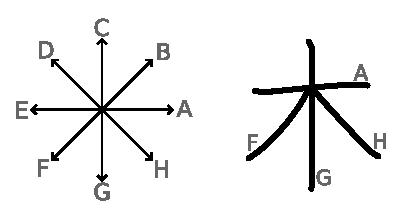
\includegraphics[width=1.75in]{./fig/stroke-categories.eps}
		\caption{A stroke may be classified according to its directionality.
			Further classes may be used to differentiate between long and short strokes,
		or to accomodate for ``pen-up'' motions. Here, the strokes of the kanji ``ki'' (tree) are identified as A-G-F-H.}
		\label{fig_stroke_categories}
	\end{figure}



	\section{Proposed solution}
	\label{sec:proposed_solution}

	%Taking into consideration the issues presented in section \ref{sec:problem_description}
	Taking the issues presented in section \ref{sec:problem_description} and the many influential works reviewed in section \ref{sec:previous_work}
	into consideration, an attempt is made to define a general description of a flexble, modular 
	design scheme that splits the identification task into coarse and fine phases---thereby reducing the complexity of each undertaking---and 
	additionally permits replacing the normalization, segmentation, and classification strategies. %, and facilitates the parallelization of fine classification.
	The design scheme is applicable to systems performing online as well as offline recognition tasks.

	\begin{figure}[b]
		\centering
		
\includegraphics[width=2.75in]{./fig/model-overview.eps}
		\caption{The model consists of five components: input normalization methods, a feature extractor,
			a clustering strategy, a router (coarse classifier), and a fine-grained classifier.}
		\label{fig_model_overview}
	\end{figure}


	
	\subsection{Input normalization}

	Improving the input data, especially by making it more uniform with respect to available training data, has the potential
	to greatly increase recognition rates. In the case of offline input, techniques include noise reduction,
	cropping, and scaling; for online input, strokes may be analyzed and altered on-the-fly to increase consistency.
	Other possibilities include blurring or otherwise distorting input data in order to generalize it. \cite{razzak2009combining}



	\subsection{Feature extraction}

	The feature extraction algoritm should take online, offline, or combined input and rapidly generate
	an n-dimensional vector representation of the provided data. The output should be sufficient for the
	routing component to reliably distinguish within which candidate subset the fine classifier should search.

	Generally speaking, a higher feature vector dimensionality would allow for the construction of more finely-tuned clusters,
	but this might well increase the likelihood of misrouting.%, resulting in a failed classification.

	Examples of feature extractors include recursive substroke segmentation and image gradation, both outlined in \cite{tanaka1999hybrid}.



	\subsection{Category clustering}

	By structuring the search space into clusters of similar categories based on extracted features, we may
	then construct a corresponding number of fine classifiers that need only concern themselves with distinguishing
	between the categories within their own clusters. Partitions could either be mutually exclusive or contain some degree of overlap.

	K-means clustering is often employed for this type of partitioning task, as is the LGB algorithm. \cite{yang2003accelerating}
	%It is worth mentioning that optimally allocating $n$ elements in $k$ partitions is an NP-hard problem, even in the case of $k = 2$. \cite{drineas2004clustering}

	
	%This translates into significant reductions in model complexity,
	%which in turn implies both a decrease in training time
	%and the possibility of higher accuracy rates. Furthermore, given that no category overlap exists
	%between the clusters, each fine classifier may be trained in parallel, and each model may be gradually
	%improved as new training data is made available.

	%Centroid-based clustering
	%"Seeks to minimize the average squared distance between points in the same cluster"
	%goal is to choose k centers so as to minimize $\varphi$, the total squared distance between each point and its closest center.

	\subsection{Routing}

	Acting upon the vector provided by the feature extractor, the router---or coarse classifier---should indicate
	within which partition the category corresponding to the input is most likely located. This component could
	be contrived to indicate not only one but multiple targets in order to dampen the effect of erroneous routing.

	A 2014 publication by Zhu and Nakagawa documents the use of genetic algorithms to programmatically generate robust coarse classifiers. \cite{zhu2014robust}


	\subsection{Fine-grained classification}

	The final and most crucial component of the system is the fine classifier, which is tasked with matching the
	given input against the candidates within its partition. As mentioned in section \ref{sec:previous_work}, a great
	variety of techniques exist, including support vector machines, Bayesian networks, hidden Markov models, and artificial neural networks.
	This step is not necessarily limited to using only one method; provided a reliable means of integration is developed,
	multiple classifiers could work in unity to provide the best possible classification.
	%As with the coarse classifier, this component could leverage either of or both online and offline information.



	\section{Experiments \& preliminary results}
	\label{sec:experiments}

	Based on the design scheme outlined in the previous section, we are currently in the process of implementing 
	a basic online kanji recognition system which we aim to evaluate on established testing benchmarks
	as well as in the form of a mobile application. The diagram in figure \ref{fig_experimental_implementation} 
	explains how the components interact.

	\begin{figure}
		\centering
		
\includegraphics[width=2.75in]{./fig/experimental-implementation.eps}
		\caption{Experimental implementation. The input is first analyzed by the coarse classifier, resulting in the G-H-A\ldots feature representation.
		Thereafter, the routing network selects which cluster to search in, and the image data is passed to the corresponding CANN for fine-grain classification.}
		\label{fig_experimental_implementation}
	\end{figure}


	\subsection{Input normalization}

	Initially, two alternatives are being explored: an approach in which no input normalization is be applied, and one 
	in which the effect of rectifying online strokes by altering or discarding points below a certain threshold is evaluated.


	\subsection{Feature extraction}

	With the intent of progressively improving the various facets of the system,
	our first feature extractor was made as simple as possible: each stroke is directly
	classified with a letter as illustrated in figure \ref{fig_stroke_categories} based solely
	on its start and endpoints. Table \ref{tbl_stroke_analysis} contains a summary of the
	result of classifying the 6,400 elements in the KanjiVG dataset in this manner.
	We speculate that excluding pen-up motions will result in a more error-resilient system.

	Additional experiments will include distinguishing between long and short strokes,
	including pen-up motions, and segmenting strokes into substrokes before classification.


	\begin{table}[b]
		\renewcommand{\arraystretch}{1.3}
		\caption{Stroke type frequency distribution overview }
		\label{tbl_stroke_analysis}
		\centering
		\begin{tabular}{ c | c c c c c l }
			\hline
			  & \bfseries \% & \small $\sum$ & $\mu$ & $\sigma$ & Highest count \\ 
			\hline
			\hline
			\bfseries A & $33.20\%$ & $26,160$ & $4.09$ & $2.33$ & $15$ & \\%(蠶) \\
			\bfseries B & $1.47\%$  & $1,159$  & $0.18$ & $0.40$ & $2$  & \\%(摑) \\
			\bfseries C & $0.00\%$  & $0$      & --     & --     & --   & \\%     \\
			\bfseries D & $0.00\%$  & $0$      & --     & --     & --   & \\%     \\
			\bfseries E & $0.31\%$  & $245$    & $0.04$ & $0.19$ & $2$  & \\%(霪) \\
			\bfseries F & $12.72\%$ & $10,018$ & $1.57$ & $1.36$ & $10$ & \\%(鏐) \\
			\bfseries G & $29.98\%$ & $23,616$ & $3.69$ & $1.96$ & $13$ & \\%(鱸) \\
			\bfseries H & $22.32\%$ & $17,587$ & $2.75$ & $1.61$ & $11$ & \\%(靆) \\
			\hline
			            & $100.00\%$   & $78,785$ &        &        &      & \\
			\hline
		\end{tabular}
	\end{table}


	\subsection{Category clustering}

	Equipped with their respective feature vectors, the 6,400 categories were partitioned into 50
	mutually exclusive clusters using the K-means++ algorithm. \cite{arthur2007k}
	Based on the information provided
	in table \ref{tbl_stroke_analysis}, only the five dimensions A, B, F, G, and H were utilized as sorting parameters.
	The number of clusters was determined empirically, using Mardia's rule of thumb \mbox{$k \approx \sqrt{n / 2}$} \cite{mardia2005multivariate}
	as an upper limit.
	

	%\begin{table}
	%	\renewcommand{\arraystretch}{1.3}
	%	\caption{Some form of cluster sample}
	%	\label{tbl_sample_clusters}
	%	\centering
	%	\begin{tabular}{c}
	%		We could list centroid info and some sample kanji. \\
	%		But not \emph{all} the clusters\ldots TMI. \\
	%	\end{tabular}
	%\end{table}


	\subsection{Routing}

	Initially, three simple routing schemes are being applied: a lookup table, a function that
	identifies the most similar centroid, and a feedforward neural network. One auxiliary goal
	at this stage---in particular with the ANN---is creating some degree of resilience to errors
	such as a missing or incorrectly traced strokes.


	\subsection{Fine-grained classification}

	We are currently designing and evaluating convolutional neural networks to perform final, visual comparisons.
	Convolutional neural networks are known to provide a measure of resilience against translation and rotation,
	thus lending themselves well to the task of offline character recognition.
	
	As previously stated, the comparatively small set of candidates (in current experiments averaging 128 kanji)
	implies that each cluster model require a lower degree of complexity. Furthermore, our expectation is that---seeing
	how each partition is likely to contain many similar-looking characters---the networks will be more likely
	to correctly discern between more minute differences that might have been generalized away in a larger-scale network.

	Finally, by focusing solely on offline recognition at this stage, we may utilize a significantly larger body of 
	training data, such as the ETL character database, which contains hundreds of thousands of handwritten kanji samples. \cite{yamamoto1986recognition} 



	\section{Future work}
	\label{sec:future_work}

	The experiments documented in this paper are an initial attempt at implementing the outlined design methodology---
	numerous venues still remain to be explored. With regard to online recognition, for instance, the feature extraction
	strategy could be enhanced to break strokes into substrokes, diffentiate between long and short strokes, and take
	pen-up movements into account. This alteration would allow for clustering on up to 25 dimensions, rather than the currently used 5.

	By substituting the current coarse classifier with an offline feature extraction strategy, the entire system could
	be applied to exclusively offline handwriting recognition tasks, such as OCR of scanned documents.

	At the CANN recognition level, there is ample opportunity both to tweak the network topology and to 
	to apply a variety of best practices \cite{simard2003best} in order to enhance the final, fine--grain recognition results.

	By developing and interchanging a series of new, differing components, we ultimately hope to validate the design scheme described in section \ref{sec:proposed_solution}. 


	\section{Summary}
	\label{sec:summary}

	In this paper we provide a general formulation of kanji handwriting recognition systems that encompass a wide range
	of techniques and use cases, based on an evaluation of the properties and problematics presented by the Japanese writing system,
	and the review of multiple designs in a corpus of prior work. We also describe our ongoing efforts
	of applying this design scheme to a basic recognition system, which we aim to continue iterating upon in future works.



	% References
	\bibliography{./references}

\end{document}
